\documentclass[tikz,border=2pt]{standalone}
\usepackage{amsmath,amssymb}
\usepackage{tikz}
\usetikzlibrary{arrows.meta}

\begin{document}
% Rationals a/b between 0 and 1 with small denominators: between any two of them there is
% always another one (density), although they do not fill the line.
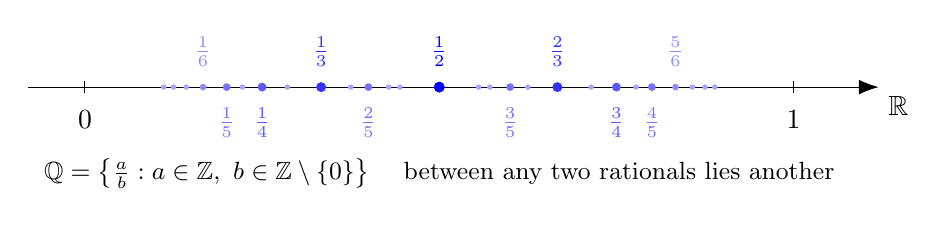
\begin{tikzpicture}[x=9cm]
	\draw[-{Latex[length=2.5mm]}] (-0.08,0) -- (1.12,0) node[below right] {$\mathbb{R}$};
	\foreach \x in {0,1} {\draw (\x,0.08) -- (\x,-0.08); \node[below=5pt] at (\x,0) {$\x$};}
	% denominators 2..6
	\foreach \p/\q in {1/2} {\fill[blue] ({\p/\q},0) circle (2pt); \node[blue, above=4pt, font=\small] at ({\p/\q},0) {$\tfrac{\p}{\q}$};}
	\foreach \p/\q in {1/3,2/3} {\fill[blue!80] ({\p/\q},0) circle (1.8pt); \node[blue!80, above=4pt, font=\small] at ({\p/\q},0) {$\tfrac{\p}{\q}$};}
	\foreach \p/\q in {1/4,3/4} {\fill[blue!65] ({\p/\q},0) circle (1.6pt); \node[blue!65, below=4pt, font=\small] at ({\p/\q},0) {$\tfrac{\p}{\q}$};}
	\foreach \p/\q in {1/5,2/5,3/5,4/5} {\fill[blue!55] ({\p/\q},0) circle (1.4pt); \node[blue!55, below=4pt, font=\small] at ({\p/\q},0) {$\tfrac{\p}{\q}$};}
	\foreach \p/\q in {1/6,5/6} {\fill[blue!45] ({\p/\q},0) circle (1.2pt); \node[blue!45, above=4pt, font=\small] at ({\p/\q},0) {$\tfrac{\p}{\q}$};}
	\foreach \p/\q in {1/7,2/7,3/7,4/7,5/7,6/7,1/8,3/8,5/8,7/8,1/9,2/9,4/9,5/9,7/9,8/9} {\fill[blue!35] ({\p/\q},0) circle (1pt);}
	\node[font=\small, align=center] at (0.5,-1.1) {$\mathbb{Q}=\left\{\tfrac ab : a\in\mathbb{Z},\ b\in\mathbb{Z}\setminus\{0\}\right\}$ \quad between any two rationals lies another};
\end{tikzpicture}
\end{document}
